\section{Methodology: A Certification Protocol for LLM Judges}

\paragraph{Why is an LLM judge needed for theorem-quality scoring?}
Evaluating AI-generated theorems/specifications requires a method to assess their quality, as proof assistants can verify a proof's correctness but not whether the agent proved the correct theorem.
This is challenging because proving the logical equivalence of two arbitrary theorem statements is generally undecidable, and an agent may generate theorems that are semantically valid but syntactically different or incomparable with the gold reference specification/theorem (e.g., by splitting a theorem into different parts).

Our goal is to certify the trustworthiness of an LLM judge for the task of formal specification/theorem generation.
This is akin to scoring the quality of a conjecture.
We operationalize this by requiring the judge to compare a candidate Lean~4 artifact (implementation, tests, theorems) against its gold-standard Lean~4 reference.
We provide the full set of Lean~4 artifacts because theorems might not make sense in isolation.
The judge returns a discrete score $s\in\{0,1,\dots,10\}$ for correctness, completeness, and semantic alignment, which we later normalize to $[0,1]$.
We use this score as a metric signal for evaluating the specifications generated by the agents.

To be considered trustworthy, the judge must satisfy the following falsifiable properties.
These are necessary conditions for trust: they certify that the judge reacts logically to structured perturbations.

\paragraph{P1 --- Identity \& Consistency.}
The judge must be idempotent at the maximum score when comparing an artifact to itself.
For any reference $X$, it must hold that $s(X,X)=1$.

\paragraph{P2 --- Monotonicity to Bugs.}
The judge's score must decrease as semantic bugs are cumulatively introduced. Let $B_1$ and $B_2$ be sets of bugs such that $B_1 \subset B_2$. For candidates $C_{B_1}$ and $C_{B_2}$ containing precisely these bug sets, the expected scores must satisfy $\mathbb{E}[s(C_{B_1})] > \mathbb{E}[s(C_{B_2})]$.

\paragraph{P3 --- Monotonicity to Missing Specs.}
The judge's score must decrease as specification elements are removed.
Let $S_1$ and $S_2$ be sets of specifications (theorems and tests) such that $S_2 \subset S_1$.
For candidates $C_{S_1}$ and $C_{S_2}$ containing precisely these specification sets, the expected scores must satisfy $\mathbb{E}[s(C_{S_1})] > \mathbb{E}[s(C_{S_2})]$.

\paragraph{Certification Protocol.}
We implement three scripted perturbation families on the \emph{candidate} while holding the \emph{gold} fixed:
(i) \emph{Identity} (P1), pairing each gold file with itself (and a semantically identical reflow) to test idempotence robustness;
(ii) a \emph{Bug Ladder} (P2), applying $k\!\in\!\{0,\ldots,K\}$ semantics-changing transformations (e.g., broken identities, violated commutativity, incorrect base cases); and
(iii) \emph{Specification Ablation} (P3), removing $m\!\in\!\{0,\ldots,M\}$ theorems or tests.
We then verify monotonicity by computing rank correlations (Kendall's $\tau$, Spearman's $\rho$) between $(k,m)$ and judged scores, and by reporting pairwise ordering accuracy (AUC) that ``worse'' artifacts receive lower scores \citep{TongZhang2024CodeJudge,Zhuo2024ICEScore}.

\textbf{Establishing trust in the LLM judge.} To ensure trustworthiness of the LLM judge in evaluating agentic autoformalization, we systematically validate key properties the judge must satisfy in Figure~\ref{fig:judge_sanity_checks}: (1) scores decrease consistently as more theorems and tests are omitted, (2) scores similarly degrade when more implementation bugs are introduced, and (3) identical file pairs always yield maximal scores.
Empirical results confirm these properties strongly hold (Pearson correlations up to $-0.973$), thus validating that our Claude~3.5-based LLM judge provides a reliable and semantically meaningful measure for correctness, completeness, and alignment of autonomously inferred theorems across \textsc{VeriBench} subsets (Table~\ref{tab:theorem_quality_table_split}) \citep{Li2024TrustLLMJudgments,Kocmi2024HumanVsLLM}.

\begin{figure*}[t]
  \centering
  \begin{subfigure}[t]{0.315\textwidth}
    \centering
    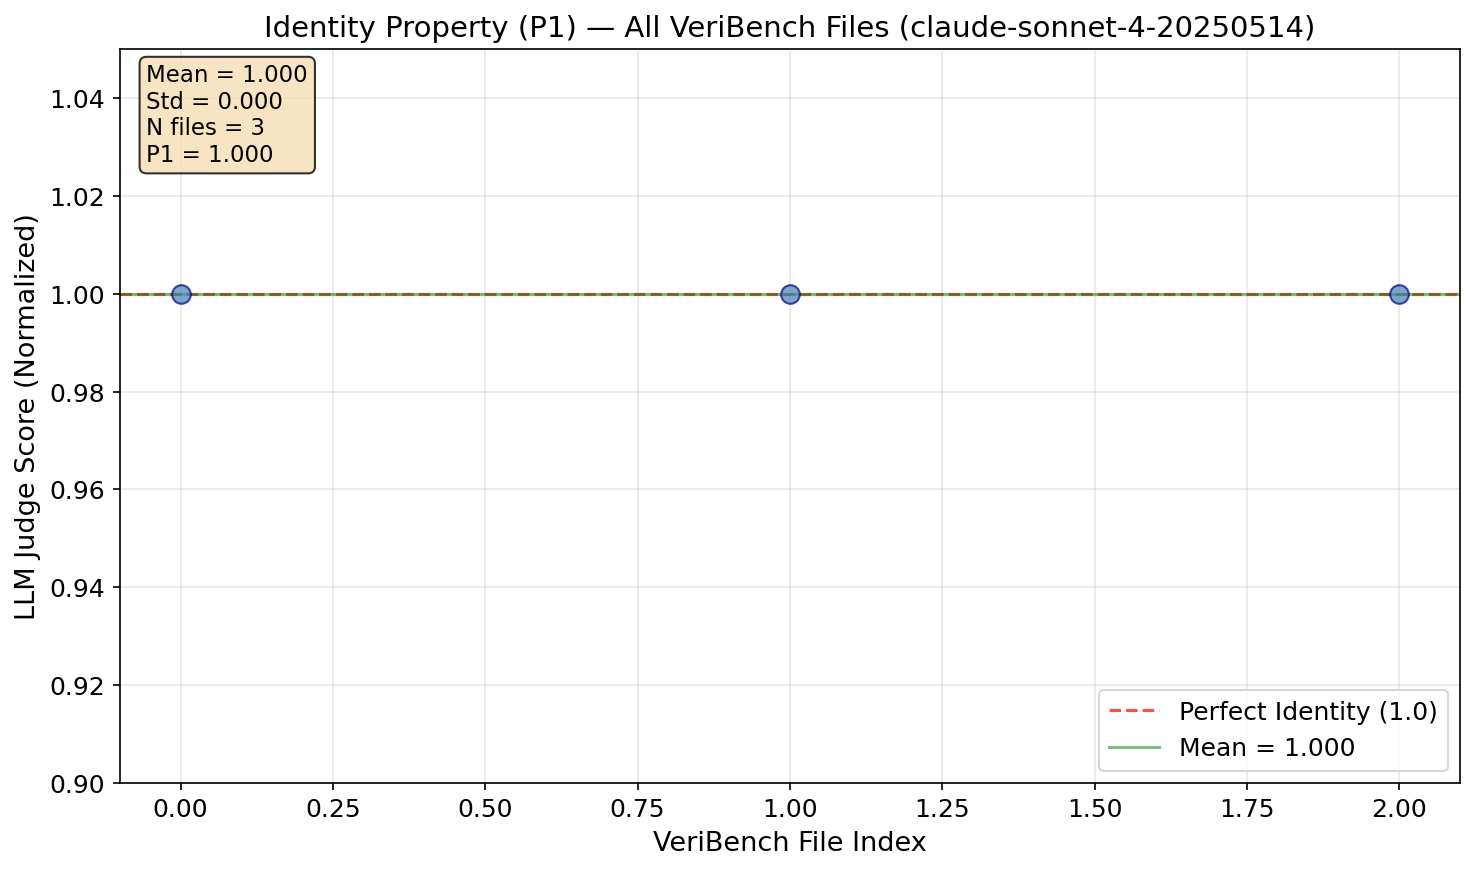
\includegraphics[width=\linewidth]{figures/identity_property.png}
    \caption{Identity (Reflexivity)}
    \label{fig:judge_identity}
  \end{subfigure}\hfill
  \begin{subfigure}[t]{0.315\textwidth}
    \centering
    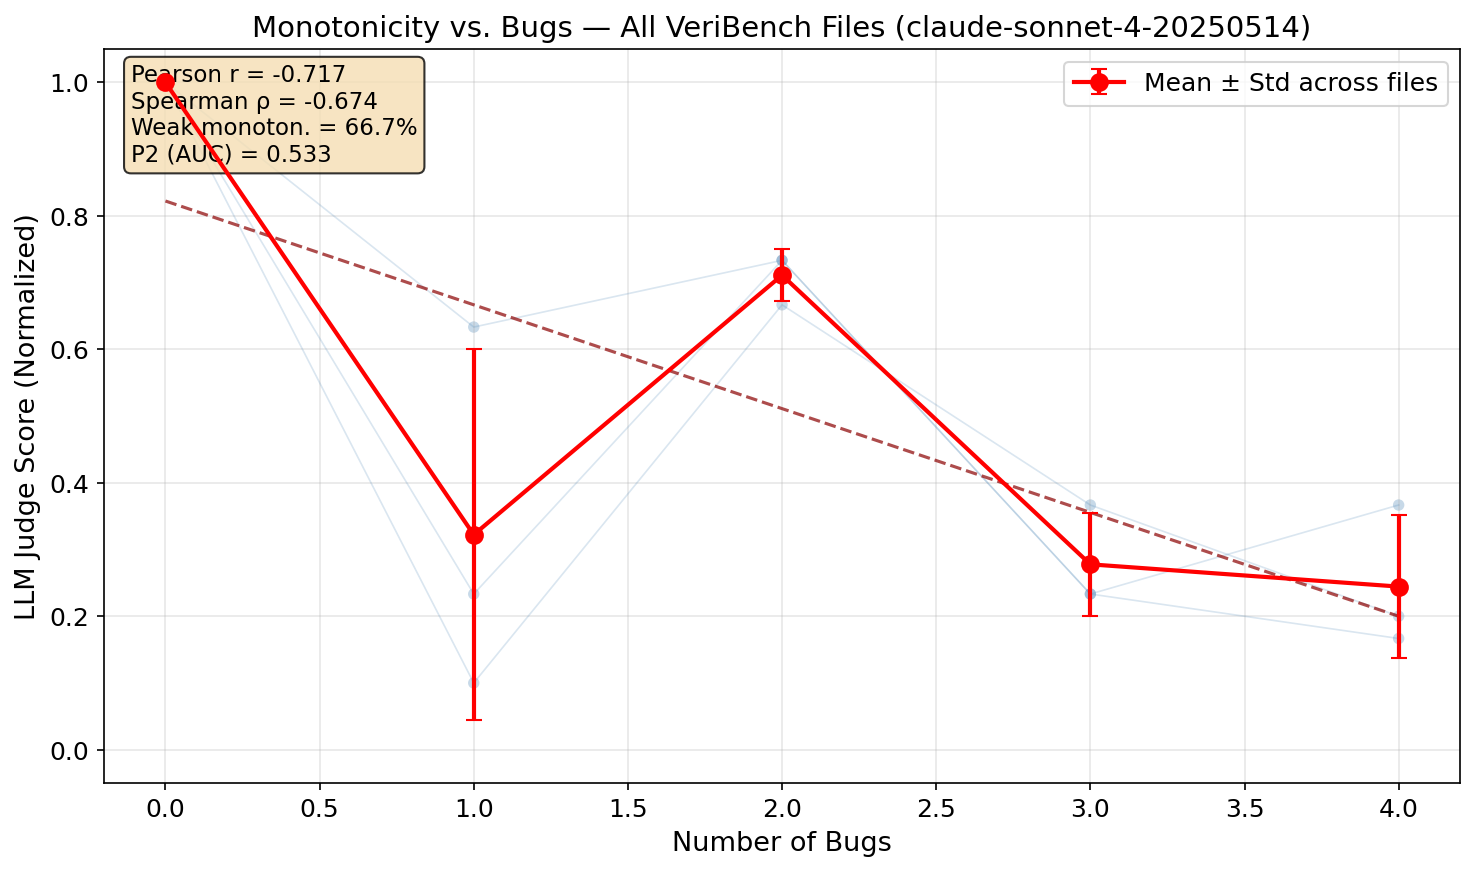
\includegraphics[width=\linewidth]{figures/monotonicity_bugs.png}
    \caption{Monotonicity vs.\ Bugs}
    \label{fig:judge_mono_bugs}
  \end{subfigure}\hfill
  \begin{subfigure}[t]{0.315\textwidth}
    \centering
    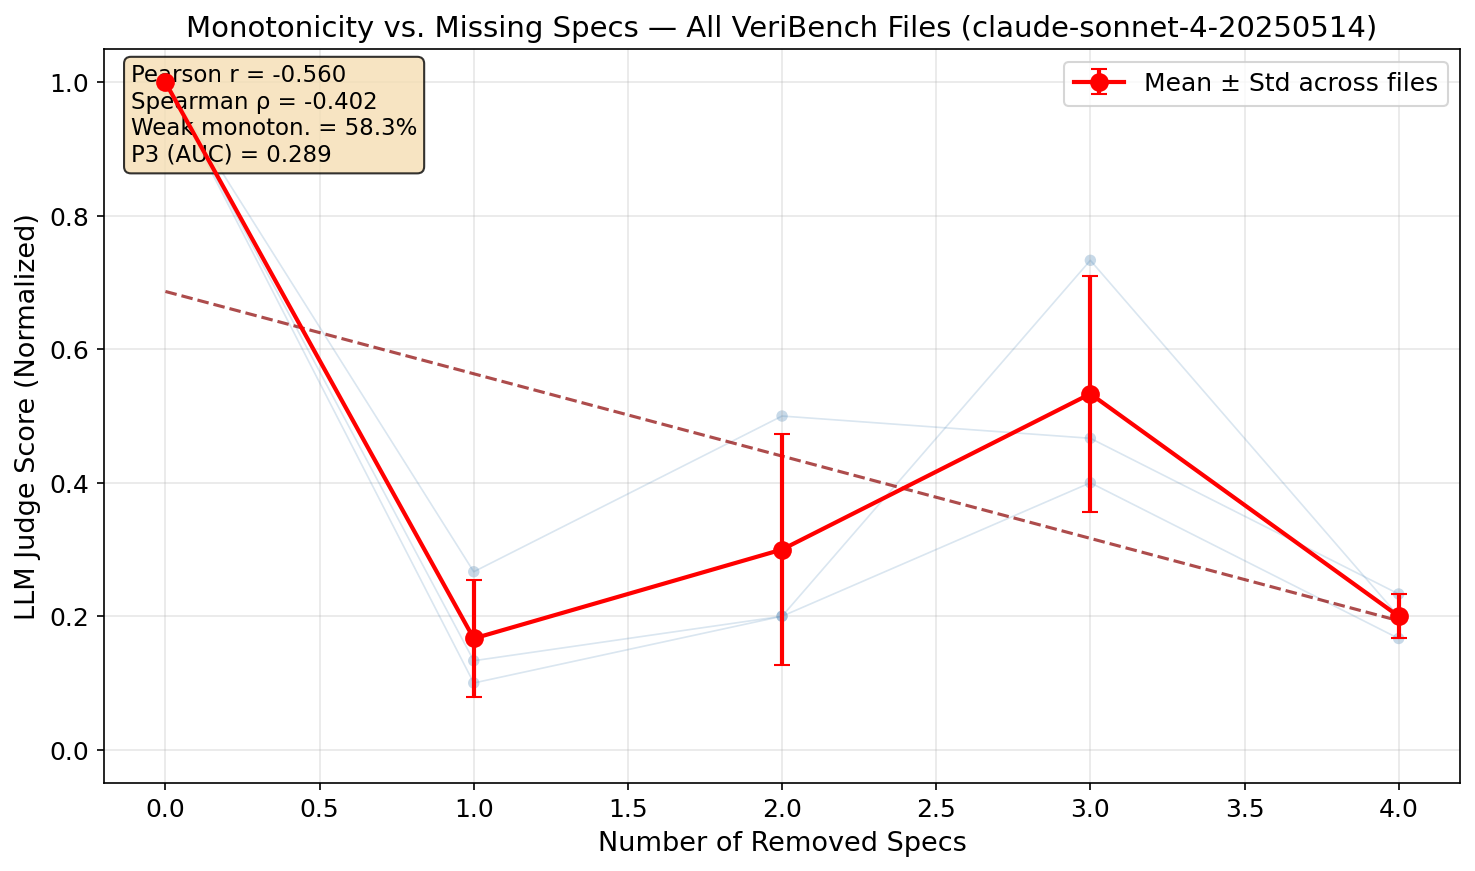
\includegraphics[width=\linewidth]{figures/monotonicity_missing_specs.png}
    \caption{Monotonicity vs.\ Missing Specs}
    \label{fig:judge_mono_specs}
  \end{subfigure}
  \vspace{-2mm}
\caption{\textbf{LLM Judge Trustworthiness Sanity Checks.}
The judge demonstrates reliability against our certification protocol.
\textbf{(a) Identity:} When comparing a gold-standard file to itself, the judge consistently returns the maximum normalized score of 1.0 ($R^2=1.000$).
\textbf{(b) Monotonicity vs.\ Bugs:} The judge's score shows a strong negative correlation with the number of injected bugs (Pearson $r = -0.973$, Spearman $\rho = -0.985$).
\textbf{(c) Monotonicity vs.\ Missing Specs:} Similarly, the score decreases predictably as specifications are removed (Pearson $r = -0.979$, Spearman $\rho = -0.985$).}
  \label{fig:judge_sanity_checks}
  \vspace{-3mm}
\end{figure*}
